% ============================================================================
% Chapter 1 — Introduction
% ============================================================================
\chapter{Introduction}
\label{ch:introduction}

% ---- 1.1 Motivation and Problem Statement -----------------------------------
\section{Motivation and Problem Statement}
\label{sec:motivation}

The pervasiveness of web-based interfaces in critical domains---healthcare portals, educational platforms, government services, e-commerce systems, and financial applications---has elevated usability and accessibility from desirable design qualities to legal and ethical imperatives. The \acrfull{WCAG}{Web Content Accessibility Guidelines} 2.2 standard codifies the technical success criteria that web content must satisfy to be perceivable, operable, understandable, and robust for users with diverse abilities. Regulatory frameworks such as the European Accessibility Act (2025), the Americans with Disabilities Act (ADA) in the United States, and Section 508 of the Rehabilitation Act increasingly mandate WCAG conformance, exposing non-compliant organisations to legal liability. According to the World Health Organisation, approximately 1.3 billion people---roughly 16\% of the global population---live with some form of disability, making accessible web interfaces not merely a compliance obligation but a fundamental prerequisite for digital inclusion.

Despite the clear importance of web accessibility, empirical studies consistently reveal widespread non-compliance. The WebAIM Million report, which annually evaluates the home pages of the top one million websites, found an average of 56.8 detectable \acr{WCAG} failures per page in its 2024 analysis, with 95.9\% of pages containing at least one automatically detectable error. These figures likely underestimate the true scope of the problem, as automated tools can only detect approximately 30--40\% of \acr{WCAG} violations; the remainder requires manual inspection by trained evaluators who understand how diverse users actually experience web content.

\subsection{Limitations of Existing Approaches}

The current landscape of accessibility and usability evaluation can be broadly categorised into three paradigms, each exhibiting fundamental limitations that motivate the work presented in this thesis.

\paragraph{Static Rule-Based Checkers.}
Tools such as axe-core, Google Lighthouse, and WAVE operate by parsing the \acrfull{DOM}{Document Object Model} and applying pattern-matching rules derived from \acr{WCAG} success criteria. For instance, axe-core checks whether every \texttt{<img>} element possesses an \texttt{alt} attribute, whether form inputs have associated \texttt{<label>} elements, and whether colour contrast ratios meet minimum thresholds. While these tools are fast, deterministic, and scalable, they suffer from three critical limitations. First, they evaluate the page as a static artefact and cannot assess dynamic behaviours that emerge during interaction---for example, whether a modal dialog traps keyboard focus, whether error messages are announced to screen readers after form submission, or whether a multi-step workflow remains navigable under cognitive load. Second, their output consists exclusively of diagnostic reports: lists of violations with references to \acr{WCAG} criteria and, occasionally, generic remediation advice (e.g., ``add an \texttt{alt} attribute to this image''). They never produce executable code patches that developers can directly apply. Third, they offer no mechanism to verify whether a proposed fix actually resolves the issue without introducing new problems.

\paragraph{Manual Expert Audits.}
Professional accessibility audits conducted by \acrfull{HCI}{Human-Computer Interaction} specialists remain the gold standard for comprehensive evaluation. Expert auditors combine assistive technology testing (screen readers, switch devices, magnification software), cognitive walkthroughs, and heuristic evaluation to identify issues that automated tools miss entirely---poor information architecture, confusing interaction patterns, inadequate feedback mechanisms, and violations of users' mental models. However, expert audits are expensive (\$5,000--\$25,000 per engagement), time-consuming (typically two to four weeks per site), and produce results that reflect the perspective of a single evaluator rather than the diversity of the actual user population. A sighted expert simulating the experience of a screen-reader user inevitably introduces perspective bias, regardless of their training.

\paragraph{User Testing with Real Participants.}
Recruiting users with diverse disabilities to test web interfaces provides the most ecologically valid evaluation data. However, this approach faces prohibitive logistical barriers: recruiting participants across the full spectrum of disabilities (visual, auditory, motor, cognitive), scheduling sessions, providing appropriate assistive technology, and compensating participants all impose significant costs and timelines. Furthermore, the combinatorial complexity of testing multiple user profiles against multiple pages with multiple interaction paths makes exhaustive coverage impractical.

\subsection{The Three Gaps}

Analysing the limitations of existing approaches reveals three interconnected gaps in the current state of practice that no single tool or methodology adequately addresses:

\begin{enumerate}
  \item \textbf{Gap~1 --- Absence of Diverse User Simulation.} No existing automated tool simulates how users with different abilities, assistive technologies, experience levels, and interaction strategies actually navigate web interfaces. Static checkers evaluate code structure; they do not model the subjective experience of a screen-reader user encountering an unlabelled button, a colourblind user struggling with a red/green status indicator, or an elderly user confused by a complex multi-step form. The interaction-level issues that arise from the interplay between user characteristics and interface design remain invisible to current automation.

  \item \textbf{Gap~2 --- Absence of Code-Level Remediation.} Existing tools produce diagnostic output---violation reports, severity ratings, and textual recommendations---but never generate concrete, executable code patches. The burden of translating a diagnostic finding (e.g., ``WCAG 1.3.1: Form input missing programmatic label'') into a working fix (e.g., adding an \texttt{aria-label} attribute, wrapping the input in a \texttt{<label>} element, or restructuring the form with \texttt{<fieldset>} and \texttt{<legend>}) falls entirely on the developer. This translation step requires accessibility expertise that many development teams lack, creating a bottleneck between diagnosis and remediation.

  \item \textbf{Gap~3 --- Absence of Closed-Loop Verification.} Even when developers do implement fixes based on audit findings, no automated mechanism exists to verify that a patch actually resolves the targeted issue without introducing regressions. A fix that adds an \texttt{aria-label} to satisfy a static checker may still fail in practice if the label text is semantically meaningless, if it conflicts with an existing \texttt{title} attribute, or if the element's focus management remains broken. Without re-evaluation under realistic usage conditions, the effectiveness of remediation efforts remains unknown until the next audit cycle.
\end{enumerate}

\begin{figure}[ht]
  \centering
  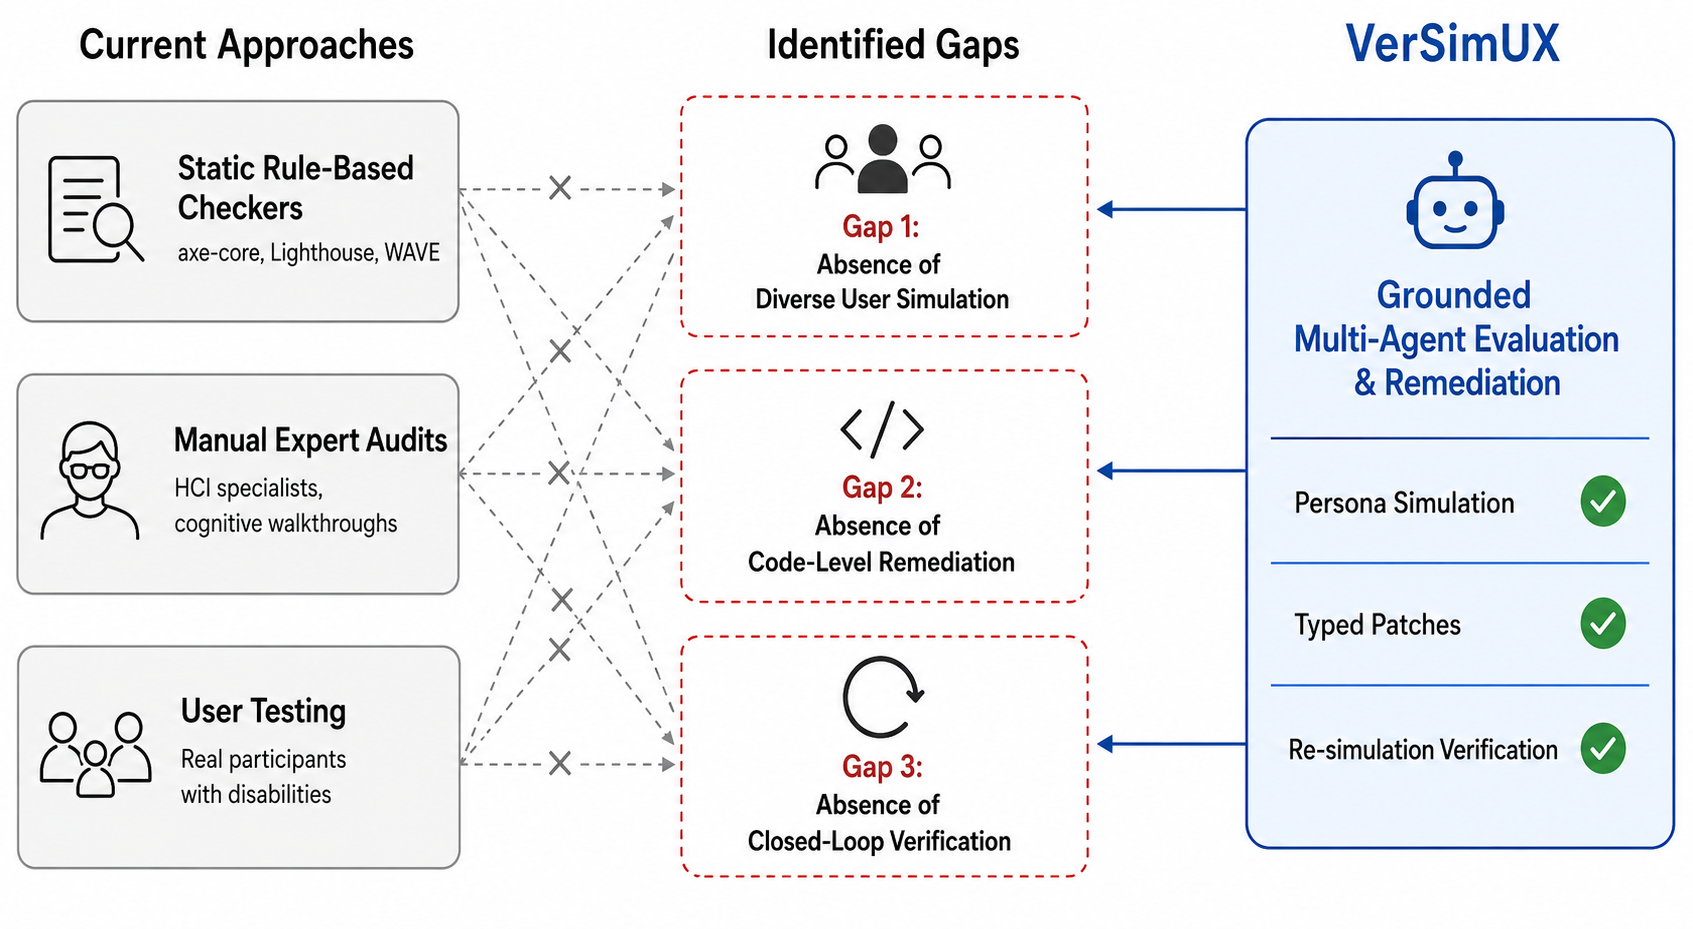
\includegraphics[width=0.92\textwidth]{static/ch01_three_gaps.png}
  \caption{The three gaps in automated web accessibility evaluation. Current approaches---static checkers, manual expert audits, and user testing---each fail to address one or more of the identified gaps. \versimux{} is designed to close all three simultaneously.}
  \label{fig:three-gaps}
\end{figure}

\subsection{Thesis Objective}

This thesis addresses all three gaps through the design, implementation, and evaluation of \versimux{}, a grounded \acrfull{MAS}{Multi-Agent System} that unifies automated diagnosis, code-level remediation, and closed-loop verification within a single orchestrated pipeline. \versimux{} operates by spawning a swarm of simulated user personas---each characterised by specific disability profiles, assistive technology configurations, technical skill levels, and behavioural tendencies---that autonomously navigate web interfaces inside real browser instances powered by Playwright. Personas execute a six-phase cognitive loop (\textit{perceive--plan--decide--execute--evaluate--reflect}) with Python-enforced grounding guards that prevent \acrfull{LLM}{Large Language Model} state hallucination, detecting usability and accessibility issues through grounded interaction rather than static analysis. A downstream pipeline of specialised agents then clusters findings using \acr{HDBSCAN} with sentence-transformer embeddings, generates typed code-level patches (HTML attributes, CSS rules, JavaScript behaviours), resolves conflicts between overlapping patches through multi-round \acr{LLM} negotiation, applies the unified patch set to the original source, and verifies the result by re-simulating failing personas on the patched interface.

The system is orchestrated as a LangGraph state graph that coordinates five specialised agent roles---supervisor, persona, recommender, conflict resolver, and verifier---across a pipeline that processes multiple pages in parallel, supports iterative correction loops, and streams real-time telemetry to a monitoring dashboard via \acrfull{SSE}{Server-Sent Events}. By grounding every evaluation in actual browser interaction and maintaining deterministic working memory in Python rather than in \acr{LLM} context, \versimux{} bridges the gap between the diagnostic capabilities of automated tools and the experiential insights of human evaluators, while producing the actionable, code-level remediation artefacts that developers need to translate findings into fixes.

\begin{figure}[ht]
  \centering
  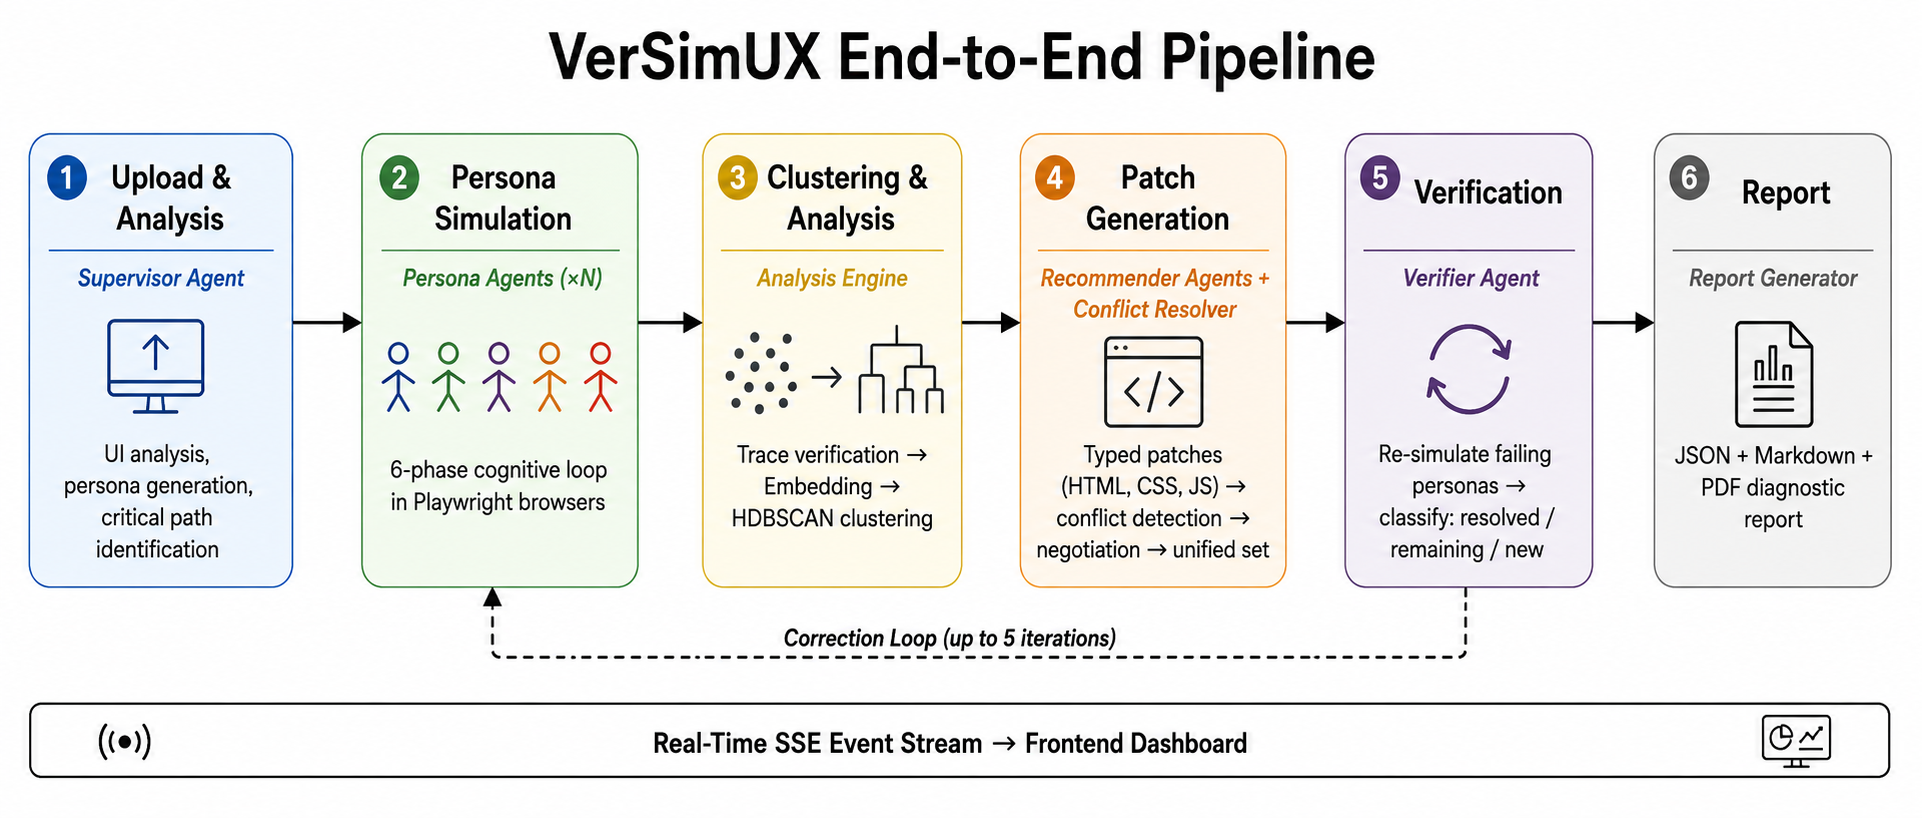
\includegraphics[width=0.95\textwidth]{static/ch01_pipeline_overview.png}
  \caption{High-level overview of the \versimux{} pipeline. HTML files are uploaded, analysed by a supervisor agent, and evaluated by a swarm of simulated personas. Findings are clustered, typed patches are generated and conflict-resolved, the unified patch set is applied, and a verification loop re-simulates failing personas to confirm effectiveness. A dashed feedback arrow indicates the iterative correction loop.}
  \label{fig:pipeline-overview}
\end{figure}


% ---- 1.2 Research Questions --------------------------------------------------
\section{Research Questions}
\label{sec:research-questions}

The three gaps identified in Section~\ref{sec:motivation} have attracted growing attention from the research community. Several recent systems have begun to explore \acr{LLM}-driven agents for interface evaluation, but each addresses only a subset of the challenges and introduces limitations that motivate the work presented in this thesis. We briefly survey five representative systems before deriving our research questions from the gaps that remain.

\subsection{Emerging Work in LLM-Based Interface Evaluation}

\paragraph{UXAgent~\cite{uxagent}.}
Xu et al. presented UXAgent at CHI~2025, an \acr{LLM} agent-based usability testing framework in which simulated users interact with live web interfaces through a browser connector. UXAgent introduces a \textit{Persona Generator Module} that synthesises diverse user profiles from researcher-defined demographic distributions, and employs dual-system reasoning---balancing fast heuristic judgements with deliberative analysis---to produce both qualitative feedback (simulated post-study surveys and think-aloud transcripts) and quantitative interaction logs. While UXAgent demonstrates that \acr{LLM} agents can approximate human-like navigation patterns and generate useful design insights, it is explicitly positioned as a \textit{study design iteration tool} rather than an end-to-end evaluation-and-remediation system. It produces unstructured diagnostic narratives but does not generate executable code patches, does not cluster or deduplicate findings across personas, and does not verify whether identified issues are resolved after intervention. Its contribution lies in demonstrating feasibility, not in closing the diagnosis-to-fix pipeline.

\paragraph{UXCascade~\cite{uxcascade}.}
Holter et al. introduced UXCascade, a scalable system that addresses the analysis bottleneck created by rapid, AI-assisted design iteration. UXCascade spins up persona-grounded \acr{LLM} agents that navigate live interfaces in parallel, records their actions and think-aloud reasoning, and---critically---aggregates unstructured agent output into a structured overview that highlights patterns across persona traits, goals, and outcomes. The system also includes an interactive fix-and-re-evaluate capability: practitioners can propose interface edits via a chat interface that generates DOM-level HTML patches, and the system automatically replays agent behaviour on the modified interface to assess impact. UXCascade thus partially addresses Gap~2 (code-level remediation) and Gap~3 (re-evaluation), but its patch generation is \textit{human-initiated}---a practitioner must manually request and review each fix through conversational interaction. The system does not autonomously generate, type, or validate patches, does not resolve conflicts between overlapping fixes, and relies on a single-shot DOM modification rather than a structured patch taxonomy. Furthermore, its re-evaluation mechanism replays the same agent trajectory rather than re-simulating under the new interface conditions, limiting its ability to detect regressions introduced by the fix.

\paragraph{ACCESS~\cite{access}.}
Huang et al. proposed ACCESS, a prompt engineering approach for automated web accessibility violation corrections. ACCESS uses the Playwright \acr{API} to systematically identify \acr{WCAG} violations, then feeds the erroneous HTML tag, error type, and violation description to a GPT model using ReAct prompting to generate corrected HTML snippets that are injected back into the \acr{DOM}. The system achieved a greater than 51\% reduction in accessibility violation errors on its benchmark dataset, demonstrating that foundation models can produce meaningful remediation code. However, ACCESS operates at the level of \textit{individual DOM elements in isolation}: it corrects one violation at a time without considering inter-patch dependencies, does not cluster related issues, and does not employ conflict resolution when multiple fixes target overlapping elements. More fundamentally, ACCESS evaluates violations through static rule-based detection (the same paradigm as axe-core), not through simulated user interaction, and therefore cannot identify the interaction-level usability issues that emerge only when diverse users navigate the interface.

\paragraph{Agentic Persona Control~\cite{agenticpersona}.}
Karthikeyan et al. presented a multi-agent framework for realistic user simulation in interactive scenarios. Their key insight is that single-\acr{LLM} user simulators lack nuance in persona adherence, exhibit excessive cooperation, and struggle with state consistency over extended interactions. To address this, they decompose the simulation into three specialised agents: a \textit{User Agent} that orchestrates the interaction flow, a \textit{State Tracking Agent} that maintains structured task state to ensure coherence, and a \textit{Message Attributes Agent} that controls conversational style based on persona and task progress. Ablation studies demonstrated significant improvements in persona adherence, task completion accuracy, and behavioural realism compared to monolithic baselines. While this work does not address web interface evaluation directly---its validation domain is restaurant ordering dialogues---it establishes an important architectural principle that \versimux{} adopts: \textit{separating cognitive concerns across specialised agents with explicit state tracking in code rather than in \acr{LLM} context} substantially improves the reliability and groundedness of persona-driven simulation.

\paragraph{AgentA/B~\cite{agentab}.}
Finally, AgentA/B automates web A/B testing by generating diverse persona-driven \acr{LLM} agents that interact with live web pages through an environment parsing module (which simplifies complex pages into structured JSON) and an action execution module (which uses browser automation to execute agent decisions). In a controlled experiment on Amazon.com involving 1,000 agents, the system demonstrated that agent behavioural trends across \acr{UI} variants were consistent with parallel human studies, though agents were more goal-directed and produced shorter action sequences. AgentA/B validates the principle that \acr{LLM} agent swarms can serve as scalable proxies for human user populations, but its focus is on comparative preference testing (which design variant performs better?) rather than diagnostic evaluation (what specific issues exist and how can they be fixed?). It does not perform accessibility evaluation, does not generate remediation patches, and does not include a verification loop.

\subsection{Remaining Gaps}

Table~\ref{tab:related-gaps} summarises the coverage of each system against the three gaps identified in Section~\ref{sec:motivation}. No existing system simultaneously addresses all three: diverse persona-driven simulation with grounded browser interaction, autonomous typed patch generation with conflict resolution, and closed-loop verification through re-simulation.

\begin{table}[ht]
\centering
\caption{Coverage of the three gaps by recent related systems.}
\label{tab:related-gaps}
\small
\renewcommand{\arraystretch}{1.2}
\begin{tabular}{@{}lccc@{}}
\toprule
\textbf{System} & \textbf{Gap 1: Simulation} & \textbf{Gap 2: Patches} & \textbf{Gap 3: Verification} \\
\midrule
UXAgent              & \checkmark & ---         & ---         \\
UXCascade            & \checkmark & Partial$^*$ & Partial$^\dagger$ \\
ACCESS               & ---         & \checkmark  & ---         \\
Agentic Persona      & \checkmark$^\ddagger$ & --- & --- \\
AgentA/B             & \checkmark & ---         & ---         \\
\midrule
\textbf{\versimux{}} & \checkmark & \checkmark  & \checkmark  \\
\bottomrule
\end{tabular}

\vspace{2mm}
\raggedright
\footnotesize
$^*$Human-initiated DOM edits, not autonomous typed patches.
$^\dagger$Trajectory replay, not re-simulation under new conditions.
$^\ddagger$Validated in dialogue, not web interface, domain.
\end{table}

\subsection{Derived Research Questions}

Building on the gaps that remain unaddressed by prior work, this thesis investigates the following research questions:

\begin{description}
  \item[RQ1 --- Diagnostic Coverage:] To what extent does \versimux{}'s persona-driven, interaction-grounded evaluation detect usability and accessibility issues that static rule-based tools (axe-core, Lighthouse) miss, and how does its diagnostic coverage compare to expert manual evaluation in terms of precision, recall, and F1 score?

  \item[RQ2 --- Grounding Effectiveness:] Do the Python-enforced working memory, action guards, and rule-based trace verification mechanisms---inspired by the cognitive decomposition principles of Karthikeyan et al.~\cite{agenticpersona}---effectively prevent hallucinated diagnoses and looping behaviours while retaining genuine usability findings?

  \item[RQ3 --- Remediation Quality:] Does \versimux{}'s autonomous patch synthesis pipeline---which generates typed code-level patches (HTML, CSS, JavaScript), detects inter-patch conflicts, and resolves them through multi-round \acr{LLM} negotiation---produce fixes that are syntactically valid, semantically correct, and applicable without introducing regressions, and how does its remediation rate compare to the single-element correction approach of ACCESS~\cite{access}?

  \item[RQ4 --- Closed-Loop Verification:] Does re-simulating failing personas on patched interfaces provide a reliable signal of remediation effectiveness, and does the iterative correction loop improve resolution rates compared to single-pass patch application as employed by UXCascade~\cite{uxcascade} and ACCESS~\cite{access}?
\end{description}


% ---- 1.3 Contributions -------------------------------------------------------
\section{Contributions}
\label{sec:contributions}

This thesis makes the following contributions, each addressing one or more of the research questions formulated in Section~\ref{sec:research-questions}:

\begin{enumerate}
  \item \textbf{A grounded persona simulation architecture (RQ1, RQ2).} We design and implement a persona agent that executes a six-phase cognitive loop---\textit{perceive, plan, decide, execute, evaluate, reflect}---inside isolated Playwright browser contexts. Each persona is characterised by a disability profile, assistive technology configuration, technical skill level, and behavioural tendency. Crucially, the agent's working memory (page phase, fields filled, steps remaining, action history) is maintained entirely in Python data structures and injected into every \acr{LLM} prompt, ensuring that the model cannot hallucinate or contradict its own state. This design directly operationalises the cognitive decomposition principle established by Karthikeyan et al.~\cite{agenticpersona} and extends it from dialogue simulation to grounded web interaction.

  \item \textbf{Deterministic action guards and trace verification (RQ2).} We introduce a suite of Python-enforced guards---scroll stagnation detection, repeat-action prevention, observe-spiral breaking, selector grounding verification, and navigation interception---that constrain persona behaviour within physically plausible interaction patterns. After simulation, a rule-based trace verifier applies heuristics (loop detection, missing selectors, network errors, unknown elements) to discard traces with greater than 40\% invalid steps before they propagate to downstream analysis. Unlike prompt-only guardrails, these mechanisms operate deterministically and cannot be circumvented by model output.

  \item \textbf{HDBSCAN-based issue clustering with semantic embeddings (RQ1).} Persona findings are deduplicated and grouped using sentence-transformer embeddings (\texttt{all-MiniLM-L6-v2}) and HDBSCAN clustering with dynamic \texttt{min\_cluster\_size}. Each cluster aggregates metadata---dominant severity, dominant category, affected personas, affected elements, and a representative description---producing a structured diagnostic output that is both machine-actionable and human-readable. This addresses a limitation shared by UXAgent~\cite{uxagent} and UXCascade~\cite{uxcascade}, neither of which clusters or deduplicates findings across multiple simulated users.

  \item \textbf{Typed, autonomous patch synthesis with conflict resolution (RQ3).} For each issue cluster, specialised recommender agents generate typed patch proposals spanning seven categories: \texttt{html\_attribute}, \texttt{html\_structure}, \texttt{content}, \texttt{css\_rule}, \texttt{css\_class}, \texttt{inline\_style}, and \texttt{js\_snippet}. When multiple patches target overlapping DOM elements, a conflict detector identifies collisions and a mediator agent resolves them through structured multi-round \acr{LLM} negotiation, producing merged or prioritised patches. This goes substantially beyond the single-element, conflict-unaware correction approach of ACCESS~\cite{access} and the human-initiated DOM editing of UXCascade~\cite{uxcascade}.

  \item \textbf{A closed-loop verification and correction mechanism (RQ4).} After patch application, a verification agent re-evaluates each original issue against the patched HTML, classifying issues as \textit{resolved}, \textit{remaining}, or \textit{new}. If the resolution rate falls below a configurable threshold (default: 80\% of critical and high-severity issues), the pipeline enters an iterative correction loop that re-simulates failing personas on the patched interface, re-clusters emerging issues, generates additional patches, and re-verifies---repeating for up to five iterations. This constitutes the first fully automated, re-simulation-based verification loop in the \acr{LLM}-driven accessibility evaluation literature.

  \item \textbf{A LangGraph-based multi-agent orchestration architecture (RQ1--RQ4).} The entire pipeline is modelled as a directed acyclic graph using LangGraph's \texttt{StateGraph}, with parallel page processing via \texttt{Send()}, type-safe state annotations with \texttt{Annotated[list, operator.add]} for concurrent write safety, and conditional edges for correction loops. This architecture coordinates five distinct agent roles---supervisor, persona, recommender, conflict resolver, and verifier---across a pipeline that scales to multiple pages and dozens of concurrent personas within a bounded thread pool.

  \item \textbf{A real-time observability and telemetry infrastructure (RQ1).} The system exposes a comprehensive event-streaming architecture based on \acr{SSE}, a thread-safe \texttt{EventBus} singleton, and a \texttt{structlog} logging bridge that automatically emits every backend log event as a structured SSE payload. Session state, events, and results are persisted to SQLite with auto-incrementing event IDs, enabling reconnection with \texttt{Last-Event-ID} tracking and full session replay after backend restarts. This infrastructure provides the observability necessary to inspect, debug, and analyse multi-agent evaluation runs in both real time and post hoc.
\end{enumerate}


% ---- 1.4 Thesis Outline ------------------------------------------------------
\section{Thesis Outline}
\label{sec:outline}

The remainder of this thesis is organised into eight chapters and four appendices, structured to move from theoretical foundations through system design to empirical validation.

\begin{description}
  \item[\Cref{ch:background} --- Background and Related Work] reviews the foundational literature across four domains: (1)~web accessibility standards and automated evaluation tools, (2)~simulated user testing and cognitive modelling, (3)~multi-agent system architectures and \acr{LLM}-based agent frameworks, and (4)~automated program repair. This chapter provides the theoretical grounding for the design decisions presented in subsequent chapters and positions \versimux{} within the existing landscape through a detailed comparison with UXAgent~\cite{uxagent}, UXCascade~\cite{uxcascade}, ACCESS~\cite{access}, and related systems.

  \item[\Cref{ch:overview} --- System Overview] provides a high-level walkthrough of the \versimux{} pipeline, from HTML upload through persona simulation, issue clustering, patch synthesis, conflict resolution, patch application, verification, and report generation. This chapter establishes the end-to-end workflow and the design principles---grounding, modularity, deterministic state management, and fail-safe degradation---that govern the architecture.

  \item[\Cref{ch:architecture} --- System Architecture] presents the detailed design and implementation of the system's core subsystems: the LangGraph pipeline topology, the supervisor agent, the persona agent with its six-phase cognitive loop and Playwright engine, the clustering engine, the recommender agent swarm, the conflict resolver, the patch applicator, the verification loop, and the report generator. Each subsystem is described in terms of its inputs, outputs, internal algorithms, and failure-handling strategies.

  \item[\Cref{ch:ai-design} --- AI and LLM Integration] discusses the \acr{LLM} integration layer in depth: prompt architecture and template design, the provider-agnostic rate limiter with per-key semaphores, the per-role \acr{LLM} router, JSON mode handling across providers, retry logic with exponential backoff, and the strategies employed to mitigate common \acr{LLM} failure modes (hallucinated selectors, malformed JSON, context window overflow, and degenerate outputs).

  \item[\Cref{ch:infrastructure} --- Runtime Infrastructure] covers the runtime environment, deployment architecture, and communication layer: the FastAPI backend with its REST and SSE endpoints, the session store with SQLite persistence and async queue broadcasting, the pipeline runner with its event mapping and heartbeat mechanism, the Playwright shared browser with thread-local caching, and the frontend dashboard architecture including the event-driven state machine and live preview system.

  \item[\Cref{ch:evaluation} --- Evaluation] presents the empirical methodology and results. This chapter describes the test corpus, evaluation metrics (precision, recall, F1 against expert baselines; patch applicability rate; regression rate; verification accuracy), experimental setup, and quantitative results for each research question. It includes ablation studies examining the contribution of individual components (grounding guards, trace verification, conflict resolution, correction loops) to overall system performance.

  \item[\Cref{ch:discussion} --- Discussion] interprets the experimental findings, analyses failure cases, discusses the limitations of \acr{LLM}-driven evaluation (model sensitivity, prompt fragility, coverage gaps for complex JavaScript-heavy interfaces), examines threats to validity, and compares \versimux{}'s performance against the related systems surveyed in \Cref{sec:research-questions}.

  \item[\Cref{ch:conclusion} --- Conclusion and Future Work] summarises the contributions of this thesis, revisits each research question with the evidence obtained, and outlines directions for future research including multi-page workflow evaluation, visual regression testing integration, fine-tuned domain-specific models, and extension to mobile native interfaces.
\end{description}

\noindent Four appendices provide supplementary material: \textbf{Appendix~A} reproduces the system configuration schema; \textbf{Appendix~B} lists the complete \acr{LLM} prompt templates; \textbf{Appendix~C} presents the Pydantic data model definitions; and \textbf{Appendix~D} provides annotated examples of full pipeline execution traces.

